\de{ĐỀ THI GIỮA HỌC KỲ I NĂM HỌC 2023-2024}{THPT GIA ĐỊNH}
%Câu 1...........................
\begin{bt}%[0D1B3-4]%[Dự án đề kiểm tra Toán 10 GHKI NH23-24- Thy Nguyen Vo Diem]%[THPT Gia Định]
	Cho các tập hợp con của $\mathbb{R}$ được xác định như sau $A=[-3;4]$, $B=(-\infty;-3] \cup [2;7)$. Tìm $A \cap B$; $A \cup B$; $A \setminus B$; $B\setminus A$.
	\loigiai{
	$A \cap B=\{-3\} \cup [2;4]$;\\
	$A \cup B=(-\infty;7)$;\\
	$A \setminus B=(-3;2)$;\\
	$B \setminus A=(-\infty;-3) \cup (4;7)$.
	}
\end{bt}

%Câu 2...........................
\begin{bt}%[0D1K3-5]%[Dự án đề kiểm tra Toán 10 GHKI NH23-24- Thy Nguyen Vo Diem]%[THPT Gia Định]
	Một nhóm có 12 học sinh chuẩn bị cho hội diễn văn nghệ. Trong danh sách đăng kí tham gia tiết mục múa và tiết mục hát của nhóm đó, có 5 học sinh tham gia tiết mục múa và 3 học sinh tham gia cả hai tiết mục. Hỏi có bao nhiêu học sinh của nhóm tham gia tiết mục hát? Biết rằng có 4 học sinh của nhóm không tham gia tiết mục nào.
	\loigiai{
	Kí hiệu $A$ là tập hợp những học sinh tham gia tiết mục múa, $B$ là tập hợp những học sinh tham gia tiết mục hát.\\
	Theo giả thiết, $n(A)=5$, $n(A \cap B)=3$.\\
	Số học sinh của nhóm có tham gia ít nhất 1 tiết mục là $n(A \cup B)=12-4=8$.\\
	Số học sinh tham gia tiết mục hát\\ $n(A \cup B)=n(A)+n(B)-n(A \cap B) \Leftrightarrow 8=5+n(B)-3 \Leftrightarrow n(B)=6$.
	}
\end{bt}

%Câu 3...........................
\begin{bt}%[0D2K2-3]%[Dự án đề kiểm tra Toán 10 GHKI NH23-24- Thy Nguyen Vo Diem]%[THPT Gia Định]
	Một xưởng sản xuất bàn và ghế. Một chiếc bàn cần $1,5$ giờ lắp ráp và $1$ giờ hoàn thiện. Bộ phận lắp ráp có 3 nhân công và bộ phận hoàn thiện có 4 nhân công. Biết thị trường tiệu thụ hết sản phẩm của xưởng và lượng ghế tiêu thụ không vượt quá $3,5$ lần số bàn. Biết một chiếc bàn lãi $600$ nghìn đồng, một chiếc ghế lãi $450$ nghìn đồng. Hỏi trong một ngày, xưởng cần sản xuất bao nhiêu chiếc bàn, bao nhiêu chiếc ghế để thu được tiền lãi cao nhất? Biết một nhân công làm việc không quá $8$ giờ mỗi ngày.
	\loigiai{
	Gọi $x$; $y$ (chiếc) lần lượt là số bàn và số ghế cần sản xuất ($x$, $y \ge 0$; $x$, $y \in \mathbb{N}$).\\
	Khi đó số tiền lãi là $f(x;y)=600x+450y$ (nghìn đồng).\\
	Số giờ lắp ráp tối đa là $8 \cdot 3=24$.\\
	Số giờ hoàn thiện tối đa là $8 \cdot 4=32$.\\
	Ta có hệ bất phương trình $\heva{&1,5x+y \le 24\\&x+2y \le 32\\&3,5x-y \ge 0\\&x \ge 0\\&y \ge 0} (*)$.
	\begin{center}
		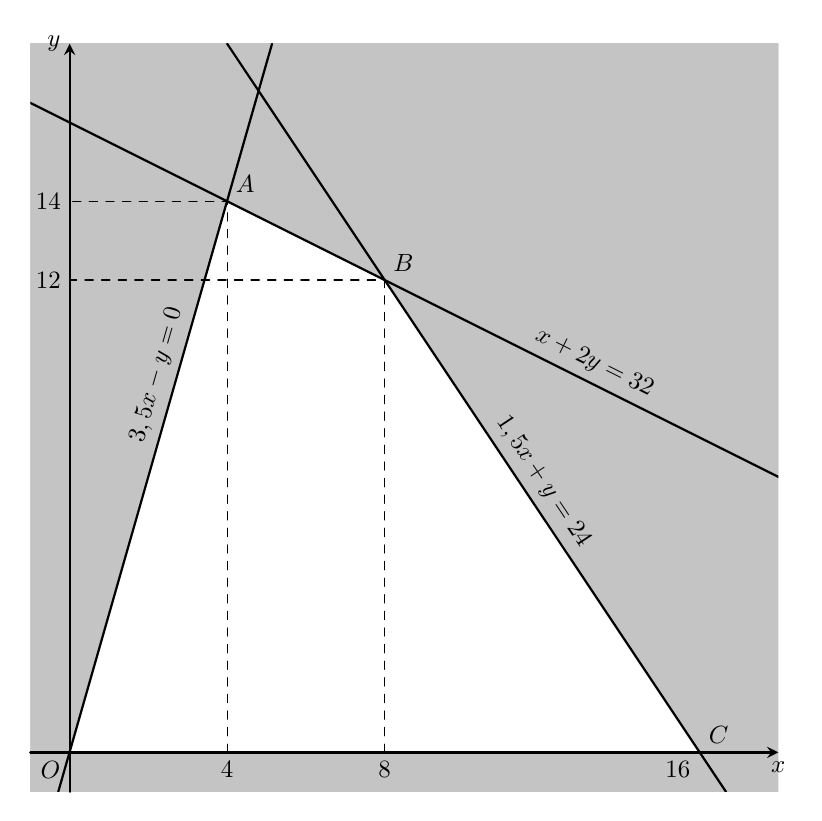
\begin{tikzpicture}[line join=round, line cap=round,>=stealth,thick,scale=0.5]
			\tikzset{every node/.style={scale=0.9}}
			\begin{scope}
				\clip (-1,-1) rectangle (18,18);
				\fill[black!23] (-2,27)--(19,27)--(19,-4.5)--cycle;
				\fill[black!23] (-5,18.5)--(35,18.5)--(35,-1.5)--cycle;
				\fill[black!23] (-2,-7)--(-2,66.5)--(19,66.5)--cycle;
				\fill[black!23] (0,-1)--(-1,-1)--(-1,18)--(0,18)--cycle;
				\fill[black!23] (-1,0)--(-1,-1)--(18,-1)--(18,0)--cycle;
				\draw (4,18)--(16.67,-1) node [pos=0.6, above, sloped] {$1,5x+y=24$};
				\draw (-4,18)--(34,-1) node [pos=0.45, above, sloped] {$x+2y=32$};
				\draw (5.14,18)--(-0.29,-1) node [pos=0.45, above, sloped] {$3,5x-y=0$};
			\end{scope}
		\draw[dashed,thin] (8,0)node[below]{$8$}--(8,12)node[above right]{$B$}--(0,12)node[left]{$12$};
		\draw[dashed,thin] (4,0)node[below]{$4$}--(4,14)node[above right]{$A$}--(0,14)node[left]{$14$};
			\draw[->] (-1,0)--(18,0) node[below]{$x$};
			\draw[->] (0,-1)--(0,18) node[left]{$y$};
			\draw (0,0) node[below left]{$O$};
			\draw (16,0) node[below left]{$16$} node[above right]{$C$};
		\end{tikzpicture}
	\end{center}
	Miền nghiệm của hệ bất phương trình $(*)$ là miền tứ giác $OABC$ (kể cả biên) với $O(0;0)$, $A(4;14)$, $B(8;12)$, $C(16;0)$.\\
	Tại $O(0;0): f(0;0)=600 \cdot 0 + 450 \cdot 0=0$;\\
	Tại $A(4;14)$: $f(4;14)=600 \cdot 4+450 \cdot 14=8700$; \\
	Tại $B(8;12)$: $f(8;12)=600 \cdot 8+450 \cdot 12=10200$;\\
	Tại $C(16;0)$: $f(16;0)=600 \cdot 16+450 \cdot 0=9600$.\\
	Ta thấy $f(8;12)$ là giá trị lớn nhất của hàm số $f(x;y)$ trên miền nghiệm của hệ $(*)$.\\
	Cần sản xuất $8$ cái bàn và $12$ cái ghế để thu về số tiền lãi lớn nhất.

	}
\end{bt}

%Câu 4...........................
\begin{bt}%[0H5B2-1]%[Dự án đề kiểm tra Toán 10 GHKI NH23-24- Thy Nguyen Vo Diem]%[THPT Gia Định]
	Cho hình bình hành $ABCD$ có $AB=5$, $AD=8$, $\widehat{BAD}=60^{\circ}$.
	\begin{enumerate}
		\item Tính độ dài $BD$ và diện tích $\triangle ABD$.
		\item Tính bán kính $R$, $r$ của các đường tròn ngoại tiếp và nội tiếp $\triangle ABD$.
		\item  Tính độ dài vectơ sau $\vec{u}=\left(\overrightarrow{CB}-\overrightarrow{CB}\right)+\overrightarrow{AD}$.
	\end{enumerate}
	\loigiai{
		\begin{enumerate}
			\item Xét $\triangle ABD$, ta có \allowdisplaybreaks{\begin{eqnarray*}
				BD^2	&=& AB^2+AD^2-2AB\cdot AD \cdot \cos \widehat{BAD} \\
					&=&5^2+8^2-2\cdot 5 \cdot 8 \cdot \cos 60^{\circ}=49  \\
			\Rightarrow	BD	&=& 7.
			\end{eqnarray*}}
		$S_{ABD}=\dfrac{1}{2}AB \cdot AD \sin \widehat{BAD}=\dfrac{1}{2}\cdot 5 \cdot 8 \cdot \sin 60^{\circ}=10\sqrt{3}$.
			\item Ta có $2R=\dfrac{BD}{\sin \widehat{BAD}} \Rightarrow R=\dfrac{BD}{2\sin \widehat{BAD}}=\dfrac{7}{2\sin 60^{\circ}}=\dfrac{7\sqrt{3}}{3}$.\\
			Nửa chu vi $p=\dfrac{5+8+7}{2}=10$.\\
			Diện tích $S=pr \Rightarrow r=\dfrac{S}{p}=\dfrac{10\sqrt{3}}{10}=\sqrt{3}$.
			\item   $\vec{u}=\left(\overrightarrow{CB}-\overrightarrow{CB}\right)+\overrightarrow{AD}=\overrightarrow{AB}+\overrightarrow{AD}=\overrightarrow{AC}$.\\
			Suy ra $\left| \vec{u}\right|=\left|\overrightarrow{AC} \right|=AC$.\\
			Ta có $\widehat{ABC}=120^{\circ}$, $BC=AD=8$.\\
			Xét $\triangle ABC$ có \allowdisplaybreaks{\begin{eqnarray*}
				AC^2	&=& AB^2+BC^2-2AB\cdot BC \cdot \cos \widehat{ABC} \\
					&=&5^2+8^2-2\cdot 5 \cdot 8 \cdot \cos 120^{\circ}=129  \\
				\Rightarrow AC	&=& \sqrt{129}.
			\end{eqnarray*}}
		Suy ra $\left| \vec{u} \right|=\left| \overrightarrow{AC}\right|=AC=\sqrt{129}$.
		\end{enumerate}
	}
\end{bt}


